The discovery of the Higgs  Boson in 2012 by CMS~\cite{Chatrchyan:2012ufa} and ATLAS
~\cite{Aad:2012tfa} experiments at the LHC open up a new era in the field of High Energy Physics. 
The Higgs Boson may only be one of the many fundamental scalar particles present in nature. 
Most extensions of the Standard Model, such as supersymmetry ~\citep{Murayama:1994kt,
Golfand:1971iw, Wess:1974tw}, predict several scalars. The two Higgs doublet model (2HDM) \cite{Branco:2011iw} which postulates the presence of an additional SU(2)$_L$ scalar doublet
is a well-motivated extension of the Standard Model. It may be considered as an effective low 
energy model of many models such as the minimal supersymmetric standard model (MSSM)
~\citep{PhysRevD.80.015017}. The model leads to very rich phenomenology and has been studied 
in considerable detail both theoretically and experimentally. 

The 2HDM postulates two scalar SU(2)$_L$ doublets with same quantum numbers. After spontaneous 
symmetry breaking it leads to five physical scalar particles out of which three are neutral 
$(H,h,A)$ and two charged $H^+$. The model can be divided into different categories depending 
on the interaction of the two Higgs doublets with quarks and leptons. 
For example, in Type I the fermions have Yukawa couplings only to the second doublet. The nature
of the Yukawa couplings determines the branching fraction of the charged Higgs into different 
final states. Here we shall be interested in the decay channel $H^+\rightarrow c\bar s$ (and its charge conjugate). The 
branching fraction for this channel ranges anywhere from 0 to 100\% depending on the choice of
Yukawa couplings for the two Higgs doublets. It depends on the parameter $\tan\beta=v_2/v_1$ 
where $v_1$ and $v_2$ are the vacuum expectation values of the two Higgs doublets. In Minimal
Supersymmetry Model (MSSM) for low values of $\tan\beta$ this is the dominant decay channel 
~\citep{PhysRevD.80.015017}. The branching ratio of charged Higgs decaying to various channel as
a function of $\tan\beta$ for different masses of charged Higgs are shown in Figure
(\ref{fig:charged_higgs_br}). 
In our analysis, we shall assume that ${\cal{BR}}(H^+\rightarrow c \bar{s}) =100$\%. 

There have been many earlier searches for charged Higgs at LEP, Tevatron, and LHC. At LEP it is
dominantly produced by the process $e^+e^-\rightarrow H^+H^-$. The search is conducted by assuming
that it decays only to $c\bar s$ and $\tau \bar \nu_\tau$. Assuming that the sum of the branching
fractions ${\cal{BR}}(H^+\rightarrow \tau^+\nu_\tau) +{\cal{BR}}(H^+\rightarrow c\bar s)=1$, a lower limit of 79.3 
\GeV is obtained for the charged Higgs mass at 95\% confidence level~\cite{Achard:2003gt,
Heister:2002ev, Abdallah:2003wd}. Under a more general assumption ${\cal{BR}}(H^+\rightarrow \tau^+\nu_\tau) 
+ {\cal{BR}}(H^+\rightarrow q\bar q)=1$, a slightly less stringent constraint of 76.3 \GeV is obtained 
at 95\% confidence level~\cite{Abbiendi:2008aa}.  

The hadron colliders at Fermilab and LHC have also imposed limits on charged Higgs parameters assuming
the production mode $t\rightarrow H^+b$. The CDF collaboration~\cite{Aaltonen:2009ke} has set 
a 95\% CL upper limit on the branching fraction ${\cal{BR}}(t\rightarrow H^+b) <10 -30$\% for the charged 
Higgs lying in the mass range $60-150$ \GeV assuming that $H^+$ decays dominantly to $c\bar s$. 
Similar limits have been obtained by the D0~\cite{Abazov:2009aa} experiment. Using the 7 TeV data,
the ATLAS collaboration has set 95\% CL upper limit on the product ${\cal{BR}}(t\rightarrow H^\pm b)\times 
{\cal{BR}}(H^\pm \rightarrow \tau^\pm\nu)< 0.23-1.3$\% for the charged Higgs mass in the range 80-160
\GeV.~\cite{Aad:2013hla}. The search for charged Higgs Boson decaying into the $c\bar{s}$ was 
performed at 8 TeV in the CMS which set 95\% CL upper limit on 
${\cal{BR}}(t\rightarrow H^+ b)$ in the range 1.2-6.5\% ~\citep{Khachatryan:2015uua}. 
The analysis presented in this note is carried out at 13 TeV with pp collision data in the CMS 
experiments recorded in 2016. The integrated luminosity of this dataset is 35.9 \fbinv.
 
%   As shown in Figure (\ref{fig:feyn_diag_sig}), for the background process one of top-quark decays to the $W^+$ 
%   and a b-quark ($t\rightarrow W^+ b$) and the other top-quark decays to $W^- \bar{b}$ ($\bar{t}\rightarrow W^-
%   \bar{b}$). Whereas for the signal process, one top-quark decays to $H^+ b$ and the other one to $W^-
%   \bar{b}$. The $W^+/H^+$ decays hadronically, whereas the $W^-$ decays leptonically. In this
%   analysis, we assume that the ${\cal{BR}}(H^+\rightarrow c \bar{s}) =100$\%. 
%   The quark-scattering diagrams have a dominant contribution to the production of top quark at Tevatron 
%   energies whereas gluon-gluon scattering diagrams are dominant at LHC energies ~\cite{Gerber:2014xea, Fiorini:2012fe}.
%     \begin{figure}
%    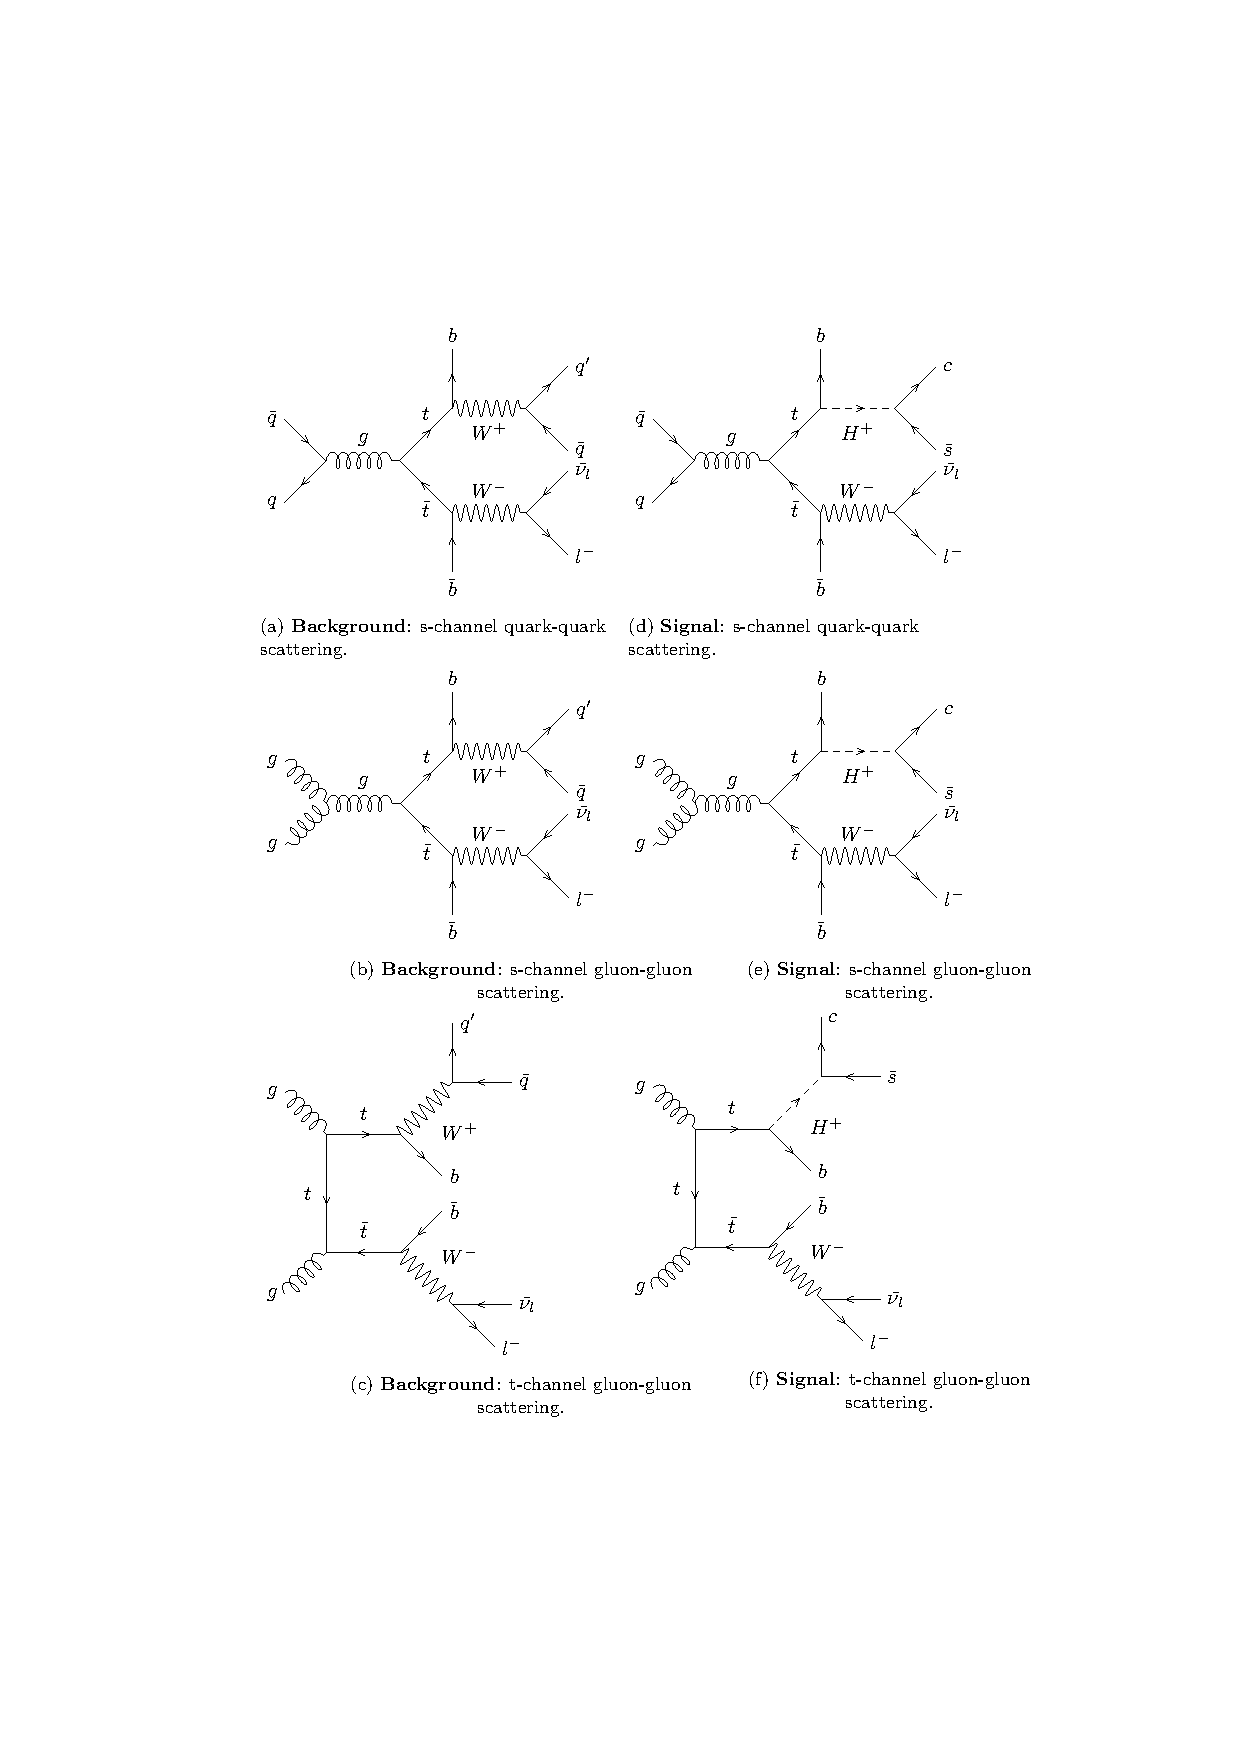
\includegraphics[width=1.0\textwidth]{Image/FeynDiag/feyn_diag_sig.pdf}
%     \caption{Production of $t \bar{t}$ from gluon-gluon and quark-quark scattering. The
%         quark-scattering production process has a dominant contribution at Tevatron energies whereas
%      gluon-gluon scattering diagrams are dominant at LHC energies ~\cite{Gerber:2014xea, Fiorini:2012fe}. The SM production
%      of \ttbar is shown in (a), (b) and (c). The charged Higgs Boson production and its decay are shown in (d), (e) and (f).}
%     \label{fig:feyn_diag_sig}
%     \end{figure}
%    
%     
\begin{figure}
    \centering  
    \subfigure[\label{subfig:CH_brs_mH100}]
    {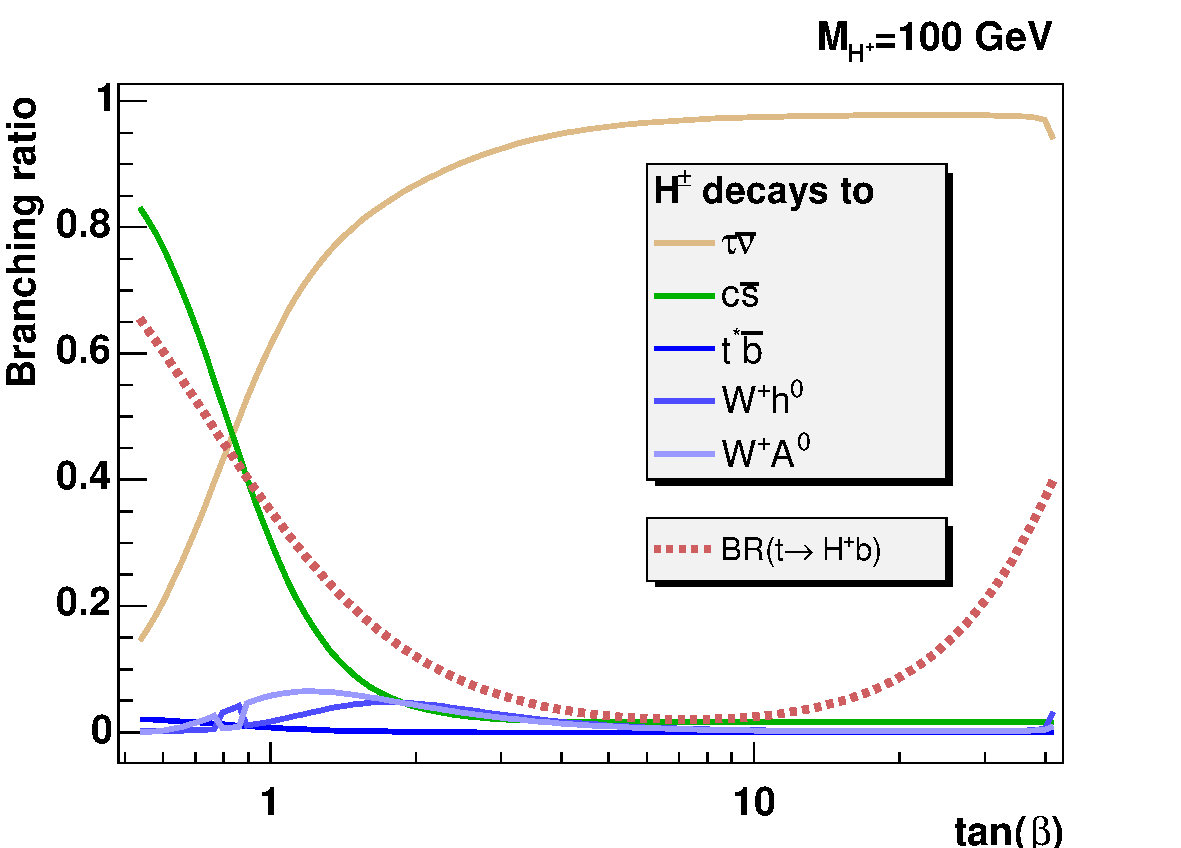
\includegraphics[width=0.50\linewidth]{Image/HplusBR/CH_brs_mH100.pdf}}
    \subfigure[ \label{subfig:CH_brs_mH120} ]
    {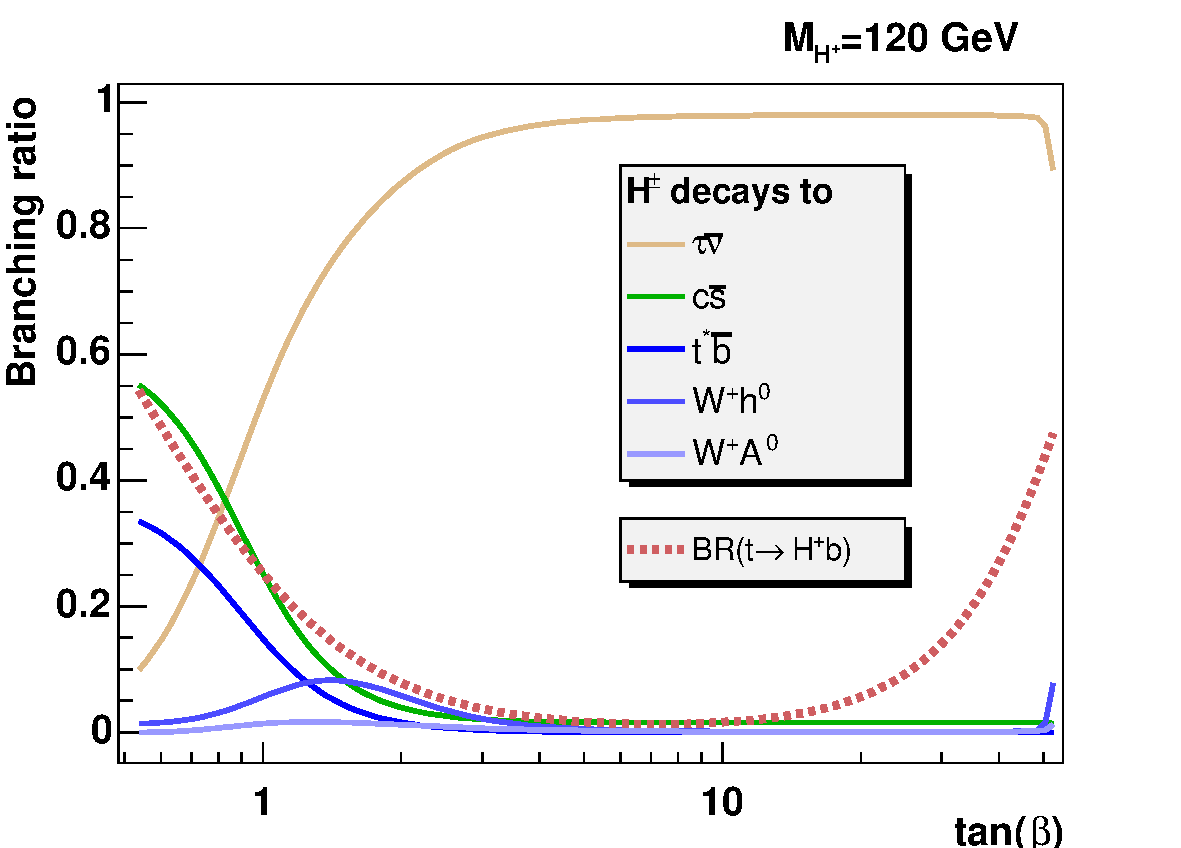
\includegraphics[width=0.50\linewidth]{Image/HplusBR/CH_brs_mH120.pdf}}
    \vfil
    \subfigure[ \label{subfig:CH_brs_mH140}]
    {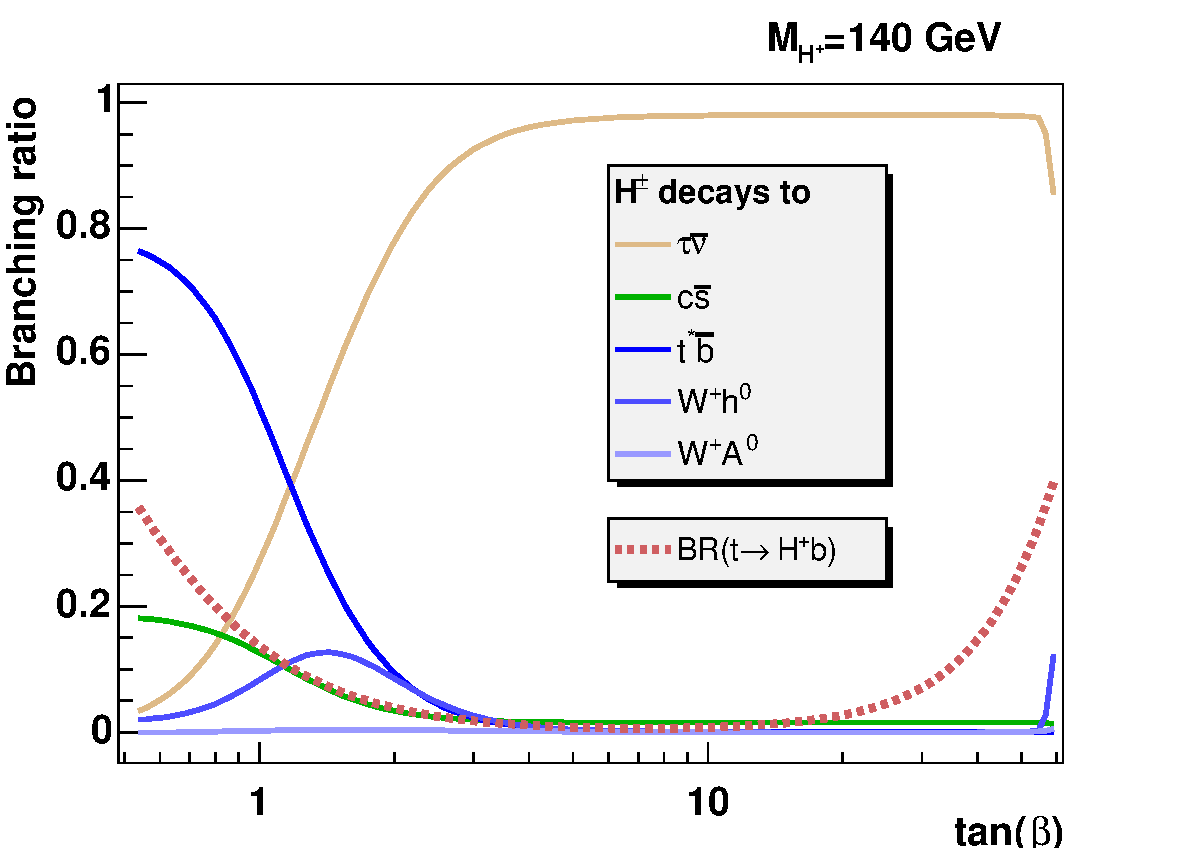
\includegraphics[width=0.50\linewidth]{Image/HplusBR/CH_brs_mH140.pdf}}
    \subfigure[\label{subfig:CH_brs_mH160}]
    {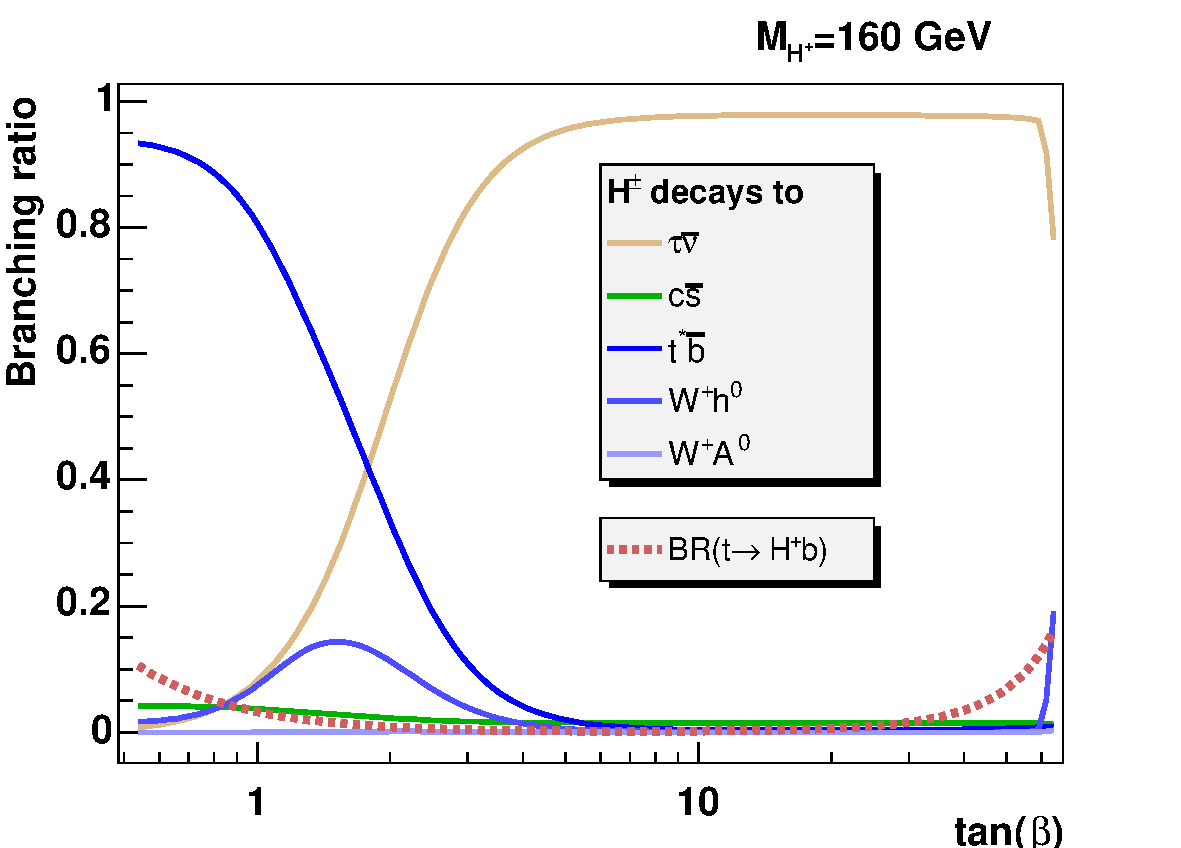
\includegraphics[width=0.50\linewidth]{Image/HplusBR/CH_brs_mH160.pdf}}
\caption{The branching ratio of charged Higgs decaying to various channel as a function of
$\tan\beta$ for different masses of charged Higgs. For low $\tan\beta$ ($<1$) the
${\cal{BR}}(H^+\rightarrow c \bar{s})$ is the dominant at lower charged Higgs masses (100 GeV, 120
GeV). However, for higher charged Higgs masses (140 GeV, 160 GeV), the 
${\cal{BR}}(H^+\rightarrow t \bar{b})$ becomes dominant for low $\tan\beta$. These figures are 
taken from~\cite{HplusBR}.}
\label{fig:charged_higgs_br}
\end{figure}

